\documentclass[%
% 	draft,
 %	submission,
  %	compressed,
  	final,
	%
% 	technote,
% 	internal,
	%submitted,
% 	inpress,
%	reprint,
%
%	titlepage,
	notitlepage,
	%anonymous,
	narroweqnarray,
	inline,
 	twoside,
%       invited,
	]{ieee}

% \newcommand{\latexiie}{\LaTeX2{\Large$_\varepsilon$}}

\usepackage[spanish,activeacute]{babel}
\newcommand{\link}[1]{\textit{#1}}


\usepackage[left=3.2cm,top=3.5cm,bottom=0.5cm,right=3.2cm]{geometry}
% \hyphenate{ad-qui-si-ci\'on}

% item bibliografico autor, titulo, descripcion
\newcommand{\ibiblio}[3]{
	\uppercase{#1} - \textbf{``#2''}, \link{#3}.
}


% para que no corte las palabras mal... no se si anda bien
\pretolerance=500
\tolerance=600

\begin{document}
\onecolumn
% \sffamily
%----------------------------------------------------------------------
% Title Information, Abstract and Keywords
%----------------------------------------------------------------------
% \title[Hardware en Argentina]{\sffamily \textbf{Desarrollos de Investigaci\'on a nivel de Hardware en Argentina}}
\title[Desarrollos de hardware en Argentina]{\sffamily \textbf{\vspace*{3cm}\\Desarrollos de Hardware \\en Argentina}}
% format author this way for journal articles.
% MAKE SURE THERE ARE NO SPACES BEFORE A \member OR \authorinfo
% COMMAND (this also means `don't break the line before these
% commands).
\author{\textbf{Ac. Kilmurray}, \textit{Gerardo Luis$^{A}$}\footnote{\textbf{A-} Departamento de Computaci\'on, Facultad de Ciencias Exactas, F\'isico-Qu\'imica y Naturales, Univ. Nac. R\'io Cuarto - Email: \small{\textit{gerakilmurray@gmail.com}} - Direcci\'on Postal: X5808DPH.} \hspace{4cm} \textbf{Ac. Picco}, \textit{Gonzalo Mart\'in$^{B}$}\footnote{\textbf{B-} Departamento de Computaci\'on, Facultad de Ciencias Exactas, F\'isico-Qu\'imica y Naturales, Univ. Nac. R\'io Cuarto - Email: \small{\textit{gonzalopicco@gmail.com}} - Direcci\'on Postal: X5800DNJ Piso 3 Dpto 6.}\\[1cm]
%         \small{\textit{gerakilmurray@gmail.com}}  \hspace{5.5cm}  \small{\textit{gonzalopicco@gmail.com}} \\ [0.5cm] 
	\large \textbf{Universidad Nacional de R\'io Cuarto}\\ \textit{Departamento de Computaci\'on}\\
	} 

\journal{Desarrollos de hardware en Argentina}
% \titletext{Estudiantes de computaci\'on Universidad Nacional de R\'io Cuarto}
 \lognumber{version 1}
% \pubitemident{S 0018--9456(97)09426--6}
\loginfo{Estudiantes de computaci\'on Universidad Nacional de R\'io Cuarto}

% \confplacedate{Ottawa, Canada, May 19--21, 1997}

\maketitle 
\vspace*{1cm}
% \begin{figure}
\begin{center}
\includegraphics[width=80pt, height=120pt]{unrc.png}\end{center} %imagen al 30 %
% \caption{Modelo Mercury Ferranti: Clementina}
% \end{figure}
\vspace*{2cm}

\begin{abstract} 

El nacimiento de los desarrollos inform\'aticos en Argentina se puede asociar con la importaci\'on de la primera computadora: Clementina. 

Dentro de los desarrollos nacionales, se destacan, proyectos acad\'emicos llevados a cabo en universidades p\'ublicas de nuestro pa\'is, tales como en la de Buenos Aires y Bah\'ia Blanca, que marcaron h\'itos en la historia de la inform\'atica.

A nivel industrial, existieron varios proyectos de empresas nacionales, que generaron muy buenos resultados, pero no perduraron mucho tiempo en el mercado. 

En el desarrollo del presente trabajo profundizaremos en proyectos, tanto a nivel industrial como acad\'emico, que mostraran las distintas situaciones abordadas por nuestro pa\'is en las diferentes etapas pol\'iticas. 

\end{abstract}
%----------------------------------------------------------------------
% SECTION: Introduction
%----------------------------------------------------------------------
\newpage
\section{Introducci\'on}

El nacimiento de las computadoras se remonta a la d\'ecada del 40, con objetivos puramente militares, con el desarrollo de una computadora denominada Z3, en 1941, por parte cient\'ificos alemanes. Mientras que Colossus, en 1944, fue desarrollada por los brit\'anicos para decodificar los mensajes cifrados de los alemanes. Casi al mismo tiempo, en los EEUU, en la Universidad de Pennsylvania, el modelo denominado ENIAC era puesto en marcha en 1946, financiada por la U.S. Army. En 1949, el Ballistic Research Laboratory (BRL) en EEUU, construye una computadora que denominaron EDVAC, la misma funcion\'o hasta 1961.

En ese momento, el acceso a las computadoras estaba restringido a cient\'ificos, ingenieros electr\'onicos y personal especializado, no solamente por sus usos militares, sino tambi\'en porque su operaci\'on era a niveles muy cercanos al hardware. Adem\'as, de que estas computadoras necesitaban un espacio f\'isico muy significativo, un consumo el\'ectrico considerable y un mantenimiento constante.

En la Universidad de Manchester bajo la direcci\'on de Tom Kilburn, se llev\'o a cabo un proyecto que ten\'ia como prop\'osito construir una computadora, que respetara la arquitectura Von Neumann. El 21 de junio de 1948, se ejecut\'o con \'exito el primer programa almacenado, en la computadora producto de este proyecto, a la cual se denomin\'o \textit{Baby}. 

En la d\'ecada del 60, la Universidad de Buenos Aires (UBA), por iniciativa y gesti\'on del Dr. Manuel Sadosky, adquiri\'o la primera computadora de la Argentina, la cual se trataba de un equipo Mercury Ferranti, de Inglaterra; la misma fue bautizada \textit{Clementina}. Este hecho marc\'o el nacimiento de las investigaciones entorno a la computadora en Argentina.\\

% \begin{figure}
\begin{center}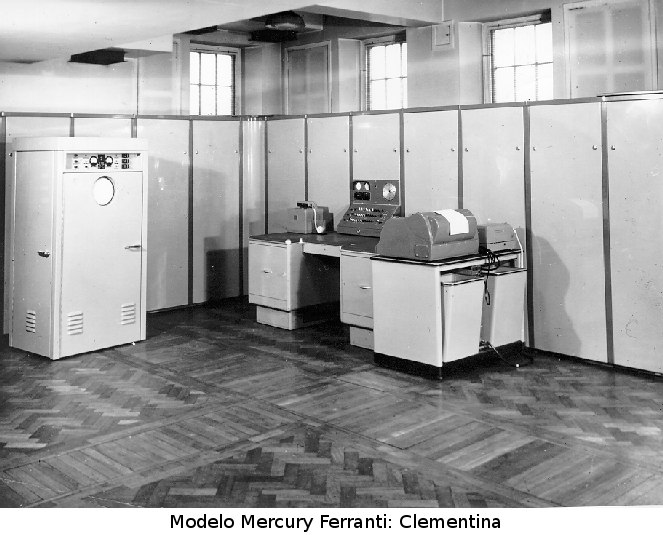
\includegraphics[width=199pt, height=161pt]{clementina.png}\end{center} %imagen al 30 %
% \caption{Modelo Mercury Ferranti: Clementina}
% \end{figure}

Sadosky, matem\'atico y cient\'ifico argentino, en 1962, impuls\'o la creaci\'on del Instituto de C\'alculo, as\'i como tambi\'en la carrera de Computador Cient\'ifico.

Cuando ya exist\'ia una masa de profesionales formados en electr\'onica digital, se encararon proyectos para construir computadoras \'integramente dentro de nuestro pa\'is. Estos desarrollos sirvieron de base para la formaci\'on de recurso humano especializado en computaci\'on digital.\\

A lo largo de este trabajo el lector podr\'a conocer proyectos nacionales, que merecen un lugar en la historia de la inform\'atica, para salvaguardarlos del paso del tiempo. El texto est\'a organizado en tres secciones: en la primera, se detallan proyectos nacionales a nivel acad\'emico, tales como, CEFIBA, CEUNS y ARGENTA. Luego, nos encontramos con una recopilaci\'on de proyectos en un marco industrial como: Serie 1000, Serie CZ, Talent y Pecos. Y por \'ultimo nos referimos a la situaci\'on actual de desarrollo de hardware, destacando a la compa\~n\'ia Novatech.



%----------------------------------------------------------------------fin----------------------------------------------------

\end{document}
